
\section{3D 프린터}

\begin{frame}{3D}

AFAS

\end{frame}


\section{3D 프린팅}

\begin{frame}{3D}
\begin{block}{}
		The “idea” of 3D printing has existed for centuries, millennia maybe.  If you look at how ancient Greeks built columns or look at François Willème 1806s work on “Photosculpture” you can see the beginnings of the idea. 
	
\end{block}
\end{frame}

\begin{frame}{FDM : Fused Deposition Modeling}

\begin{minipage}{.5\textwidth}
	\centering
		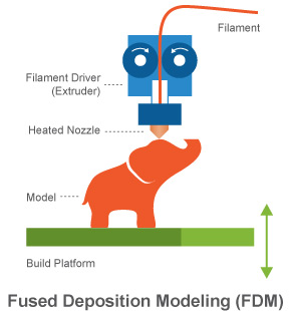
\includegraphics[width=0.8\linewidth]{images/FDM1}
	\captionof{figure}{A figure}
	\label{fig:test1}
\end{minipage}%
\begin{minipage}{.5\textwidth}
	\centering
		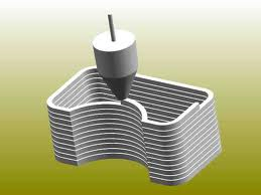
\includegraphics[width=0.8\linewidth]{images/FDM2}\textbf{}
	\captionof{figure}{Another figure}
	\label{fig:test2}
\end{minipage}

\end{frame}

